\documentclass[a4paper,10pt]{article}
\usepackage[utf8]{inputenc}
\usepackage{charter}
\usepackage{listings}
\usepackage{color}
\usepackage{url}
\usepackage{amssymb}
\usepackage{amsmath}
\usepackage{hyperref}
\usepackage{graphicx}
%\usepackage[section]{placeins}

\definecolor{grey}{rgb}{0.9,0.9,0.9}

\lstset{
language=Python,
basicstyle=\footnotesize\fontfamily{pcr},
backgroundcolor=\color{grey},
numbers=left,
numberstyle=\tiny,
numbersep=5pt,
showstringspaces=false,
tabsize=2,
breaklines=true
}

\setlength{\parindent}{0pt}

\title{Improving schedulability rate of EDF when taking into account the preemption cost in uniprocessor periodic systems}
\author{Thomas Chapeaux}
\date{Summer 2013}
%opening
\sloppy
\begin{document}
\maketitle

\tableofcontents

\newpage

\begin{abstract}

In preemptive scheduling techniques of real-time systems, a task can be interrupted during its execution to allow another task to meet its deadline. Previous results, such as the optimality of the EDF scheduler, assume that the added cost of the preemptions (including context saving and restoration, as well as the increase in cache misses) is negligible compared to the tasks execution times. In this paper, we show that within a model taking this cost into account, the optimality of EDF is no longer guaranteed. We then propose another algorithm which strictly dominates EDF in the model, and prove that it is also optimal for implicit deadline systems.

\end{abstract}

\newpage

\section{Introduction}

...

\section{Model}

    \subsection{State of the Art}

        The results presented in this section use the assumption that preemption times are negligible.\\

        We use an extension of Liu and Layland model presented in \cite{Liu:2000:RS:518501} to formalize real-time systems. This model represents such systems by a set of \textbf{tasks} generating \textbf{jobs}, where a job is a whole entity of computation with a given time of arrival and a given deadline.\\

        \subsubsection{Tasks and jobs}

        Tasks are used to model recurring jobs. They are denoted as the tuple $\tau_i = (O_i, T_i, D_i, C_i)$, where
        \begin{itemize}
            \item $i = \{1,2,...\}$ is an unique identifier for the task.
            \item $O_i$ is the minimal time at which the first job of the tasks is generated.
            \item $T_i$ is the minimal time between two job generations.
            \item $D_i$ is the relative deadline of its job.
            \item $C_i$ is the execution time of its job.
        \end{itemize}

        A task $\tau_i$ generates jobs, denoted as the tuple $J_{i,j} = (a_{i, j}, d_{i,j}, c_{i,j})$ where :
        \begin{itemize}
            \item $j = \{1,2,...\}$ is an unique identifier for the job within $\tau_i$.
            \item $a_{i,j} = O_i + (j-1) \cdot T_i$ is the arrival time (or \emph{activation time}) of the job.
            \item $d_{i,j} = a_{i,j} + D_i$ is an absolute deadline at which the job must be completed.
            \item $c_{i,j} = C_i$ is the time it takes to complete the job (\emph{execution time}).
        \end{itemize}

        We also assume a discrete time, meaning that we consider that time passes one unit (sometimes called \emph{clock tick}) at a time. This means that the values listed above must be integers and that jobs will execute for whole units.\\

        In this paper, we only consider \textbf{constrained deadline} systems, where $D_i \leqslant T_i \; \forall i$, and sometimes the particular case of \textbf{implicit deadline} systems, where $D_i = T_i$.\\

        Similarly, we differentiate between \textbf{synchronous system} (where $O_i = O_j \; \forall i,j$) and asynchronous systems (which are not synchronous).

        \subsubsection{Schedule and feasibility}

        A scheduling policy (or \emph{algorithm}) is said to be \textbf{idling} if it allows instants at which no jobs are executing even if there are released and unfinished jobs present in the system. It is said to be \textbf{preemptive} if it allows the processor to begin computation of a new job when the currently computed job is still unfinished.\\

        A system is said to be \textbf{schedulable by a scheduling policy} if it exists a scheduling policy such that every job in the task set completes before its deadline is reached. A system schedulable by at least one scheduling policy is said to be \textbf{feasible}.\\

        The authors of \cite{liu1973scheduling} have shown that the EDF (Earliest Deadline First) scheduling policy, in which jobs are prioritized according to their absolute deadline, is optimal, meaning that any feasible system is schedulable by EDF.\\

        \subsubsection{Feasibility Analysis}

        For implicit task systems, $U_{tot} \leqslant 1$ is a necessary and sufficient condition of feasibility.\\

        For (a)synchronous constrained deadline systems, $[O_{max}, O_{max} + 2 \cdot H]$ (with $O_{max}$ being the maximal task offset and $H$ the LCM of periods) is a feasibility interval for EDF.

    \subsection{Preemption Cost}

        We now consider that preemption costs are not negligible. We thus define a parameter $\alpha$, constant for all tasks of a system, called the preemption cost.\\

        Once a previously preempted job is chosen for computation by the scheduling policy, it enters an uninterruptible preemption recovery period, as seen in Fig.~\ref{fig:prp}.\\

        \begin{figure}[h]
        \begin{center}
            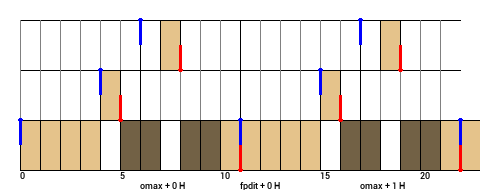
\includegraphics[width=\textwidth]{figs/atomicpreemption_example.png}
            \caption{Schedule of a system with $\alpha=2$. At t $t=6$, the preemption recovery period is not interrupted even though a job with higher priority is activated}
            \label{fig:prp}
        \end{center}
        \end{figure}

        Meumeu is FTP-optimal (equivalent to ExhaustiveFTP)

\section{Performance of EDF with preemption cost}
% Rename section to something like "Old results do not old, bitch"

    In this section, we show that the EDF scheduling policy, optimal when the preemption costs are negligible, is less adapted to our model with costly preemptions.

    \subsection{Non-optimality}

        Consider the following task system

        \begin{center}
            \begin{tabular}{|r|c|c|c|c|c|}
                \hline
                            & $O_i$ & $C_i$ & $D_i$ & $T_i$ & $\alpha_i$ \\ \hline
                $\tau_1$    & 0     & 3     & 6    & 6     & 2     \\ \hline
                $\tau_2$    & 1     & 2     & 4    & 4     & 2     \\ \hline
            \end{tabular}
        \end{center}

        When scheduled by EDF, this job miss a deadline\\

        \begin{figure}[h]
        \begin{center}
            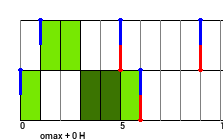
\includegraphics{figs/edfNonOptimal_EDF.png}
            \caption{A system scheduled by EDF where a deadline is missed}
            \label{fig:edfnonoptimal_edf}
        \end{center}
        \end{figure}

        However, there exists a schedule which does not miss any deadline:\\

        \begin{figure}[h]
        \begin{center}
            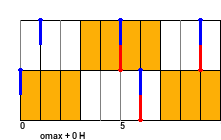
\includegraphics{figs/edfNonOptimal_PALLF.png}
            \caption{The system of Fig.~\ref{fig:edfnonoptimal_edf} with a different schedule in which no deadline is missed}
            \label{fig:edfnonoptimal_pallf}
        \end{center}
        \end{figure}

        EDF is thus non-optimal.

    \subsection{Anomalies}

        \subsubsection{Longer transitive period}
        Consider the following system

        \begin{center}
            \begin{tabular}{|r|c|c|c|c|c|}
                \hline
                            & $O_i$ & $C_i$ & $D_i$ & $T_i$ & $\alpha_i$ \\ \hline
                $\tau_1$    & 0     & 5     & 10   & 10    & 1     \\ \hline
                $\tau_2$    & 4     & 1     & 1    & 10    & 1     \\ \hline
                $\tau_3$    & 6     & 4     & 10   & 10    & 1     \\ \hline
            \end{tabular}
        \end{center}

        When scheduling this system with EDF, we see that at instant $O_{max} + 2 \cdot H$, the system has not reached a periodic behavior yet. This only happens at instant $O_{max} + 4 \cdot H$.\\

        Figure.

        \subsubsection{Deadline miss in transitive, not in periodic}

    \subsection{Other properties of constrained deadline systems}

    In this section, we present other results which do not hold under the costly preemption assumption.

        \subsubsection{Idling dominate non-idling}

        Consider the following system

        \begin{center}
            \begin{tabular}{|r|c|c|c|c|c|}
                \hline
                            & $O_i$ & $C_i$ & $D_i$ & $T_i$ & $\alpha_i$ \\ \hline
                $\tau_1$    & 0     & 3     & 8    & 8     & 2     \\ \hline
                $\tau_2$    & 0     & 3     & 5    & 8     & 2     \\ \hline
                $\tau_3$    & 1     & 1     & 1    & 8     & 2     \\ \hline
            \end{tabular}
        \end{center}

        And consider the following schedule which shows that it is feasible with an idling scheduling policy.

        [figure]

        However, it is easy to see that no non-idling algorithm can successfully schedule this system: at $t=0$, a non-idling algorithm has to choose between the first job of $\tau_1$ and $\tau_2$ for execution, whichever is chosen will then be preempted by the first job of $\tau_3$ (if not, it will miss its deadline in $t=2$). Then, at $t=2$, there will be $3+2+2=7$ units of computation left to compute before the deadline at $t=8$, the system will thus certainly miss a deadline.


        \subsubsection{Dynamic dominate fixed-job}

        \subsubsection{u < 0.69 is not sufficient}

        \subsubsection{Require Claivoyance}

        \subsubsection{Preemption can happen anywhere}

\section{PA-EDF: an extension of EDF for costly preemption}

\nocite{*}
\bibliographystyle{plain}
\bibliography{paper-paedf}


\end{document}
